\documentclass[UTF8]{book}
\usepackage{graphicx}
\usepackage{caption}
\usepackage{subcaption}
\usepackage{float}
\usepackage{amsmath}
\usepackage{seqsplit}
\usepackage{tikz}
\usepackage{pgfplots}
\usepackage{listings}
\usepackage{CJK}

\newtheorem{theorem}{Proposition}
\newcommand\longnumber[2]{%
    \begin{minipage}{#1}
    \seqsplit{#2}
    \end{minipage}
    }
\newcommand*\thickdash{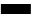
\includegraphics{thick-dash2}}
\newcommand*\thickdot{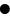
\includegraphics{thick-dot2}}

\graphicspath{ {images/} }
\begin{document}
\begin{CJK}{UTF8}{gbsn}

\title{The Network}
\author{Dan Auerbach}
\date{2015}
\maketitle

Our society sees the world through the lens of information, and this fundamental shift in our collective thinking has permeated the standard lexicon. If we are stretched thin at work, we say that we do not have enough \emph{bandwidth} to complete an extra task. If an activity will take too much time, we say that we do not have enough \emph{cycles}. We know roughly how many songs can be stored on a \emph{gigabyte} sized thumb drive, or how many \emph{megapixels} our phone's camera needs to make a good quality photo.

And while computer usage has taught a basic literacy to people all over the world about how information is stored, transferred, and processed, \emph{information theory} as a field of study has at the same time infiltrated many other academic fields of study. The elegant formulation at the core of information theory, first described by the researcher Claude Shannon in 1948, turns out to be applicable not just to understanding information in computer networks, but also to genetics, economics, molecular biology, electrical engineering, applied physics, and even abstract branches of theoretical physics and mathematics. It has become a conceptual centerpiece spanning a staggering number of disciplines. Even more amazingly, unlike previous transformative works like Isaac Newton's Philosophiæ Naturalis Principia Mathematica, Claude Shannon's core ideas are rather straight forward to understand. One of the major goals of this text is to become familiar with the basics of information theory.

Beyond the abstract theory of information, there are a host of much more practical questions that one can ask about modern information technology. How do computers work? How does the Internet work? How do phones work? How does wireless technology work? Developing a complete understanding of these questions may feel hopelessly out of reach to most readers, but this pessimism is not warranted.

To help manage this daunting array of unknowns, it helps to conceptualize questions about information technology against two broad and interrelated topics: computing and networking.

\begin{figure}[H]
\centering
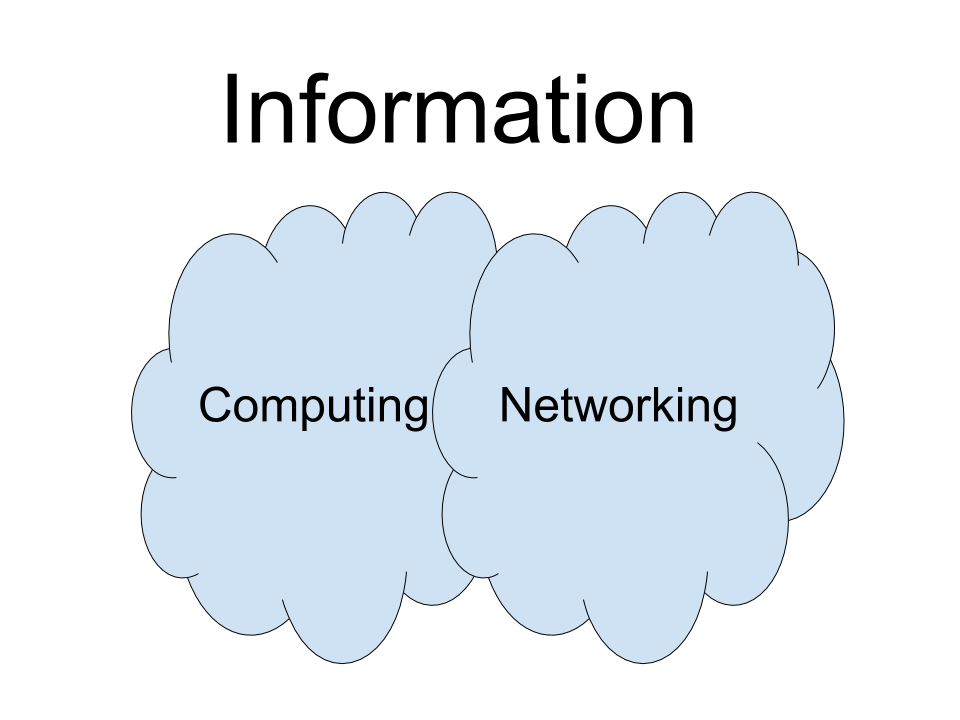
\includegraphics[width=0.9\linewidth]{information_computing_and_networking}
\end{figure}

If you learn about computing, you will learn about how your laptop works, and how your phone works (since your phone is really just a computer). You will learn about how computers can accomplish useful things like displaying a cute video of a cat on your screen. You will learn about microprocessors, random access memory, hard drives, and many other components that allow these systems to talk to one another and take input from users. You will learn about software, programming languages, how code is written, algorithms, computer graphics, Moore's law, and the limits of computing. You will learn about copyright, the battles between free and proprietary software, the role the government played in developing early computers, and the ecosystem of private companies that allow you to go to the store and buy a phone with pre-installed software.

In contrast to a course of study focused around computing, if you study networking you will learn about the ways in which computers talk to one another, and the complex systems by which information is transferred. You will learn all the dizzying steps that get that cat video onto your computer in the first place. You will learn about how your phone communicates with cell towers, what role telecommunications providers like AT\&T play, the economics of telecommunications, surveillance of communications by governments and the regulatory landscape aimed to protect ordinary users.

In practice these topics are often intertwined in thorny ways and so an individual who is interested in information will invariably learn bits and pieces of both on the journey of deepening his or her understanding.

This book focuses primarily on the networking umbrella: our goal will NOT be to understand how computing works, though that these topics are often quite intertwined, we will occasionally talk about computing. For readers without a background in computing who want an excellent practical introduction to the fundamentals of how a computer works, I strongly recommend the book \emph{Code} by Charles Petzold. For those more inclined towards the theoretical puzzles of computing, abstracted away from the hardware, a good introductory text is \emph{The Pattern on the Stone} by W. Daniel Hillis.

While this book is largely focused on networking, it is framed more broadly as a study into the role of technology in human communication throughout history. This framing will allow us to weave together technological and social history, electrical engineering fundamentals, networking, cryptography, and the theory of information.

The text is structured around five historical technologies: the telegraph, the telephone, radio, the Internet, and mobile phone. No prior technical knowledge is required. As we progress, however, the text will gradually become more technical, as we will flesh out an understanding of the following tree of topics:

\begin{quotation}
[SKILL TREE]
\end{quotation}

By the end of the book, you should have a solid understanding of all of the topics in this tree, and as we progress the book will have informal exercises for you to test your understanding. As the technical material ramps up, you will probably get more out of the book by having a pen and paper handy to solve problems as you go.

\end{CJK}
\end{document}
